This chapter covers the background areas and related work necessary to understand the contributions of this dissertation. It discusses the current state of the effort to incorporate domain knowledge in data mining. In addition, it describes the various formalisms proposed in the literature to use graphs in tackling data mining and knowledge representation problems. We conclude with a high-level summary of these background areas.

\section{Domain Knowledge in Data Mining}
Domain knowledge relates to information about a specific domain or data that is collected from previous systems or documentation, or elicited from domain experts. In the rest of the section, we highlight a body of studies that aims at exploring ways to employ domain knowledge in data mining. The results from these studies strongly attest to the positive influence of domain knowledge. Domain knowledge can affect the discovery process within a data mining system in at least two ways. First, it can make patterns more visible by generalizing the attribute values, and second, it can constrain the search space as well as the rule space.

In order to effectively summarize and compare different previously proposed systems, we propose a reference framework to classify different kinds of domain knowledge at a very high abstraction level as detailed in the following.

\begin{itemize}
\item	Knowledge about the domain: This category contains information related to a specific domain of discourse, usually obtained from either domain experts or previous data mining processes. Examples of such knowledge include concept hierarchy, integrity constraints, \etc.
\item	Knowledge about the data: This category contains information about dataset, including how it is generated, transformed and evolved. This knowledge is obtained from data producers (people who carry out experiments or collect data) or database managers. \eg, in a database of spatial information, one of the images may have been recorded with a very skew angle on the object. When processing the database the discovery process must take this information into account.
\item	Knowledge about the data mining process: This category contains information pertaining to specific data mining sessions, including goals, parameters and variables related to the experiment. \eg, attributes of interest within data, roles of attributes as being whether antecedents or consequences in association rule mining, and the measure of interestingness for discovered patterns.
\end{itemize}

The summarized work can be divided into two groups. The first group does not explicitly leverage any knowledge representation approaches to model domain knowledge. The second group explores mainly ontological knowledge (concept hierarchy) and uses formal ontology languages to encode such knowledge. The kind of domain knowledge involved in the first group is broader which covers all categories discussed in the above reference classification scheme. However, it is achieved at the cost of less formality which often result in ad-hoc expression of domain knowledge that has a very application-specific form, scop and granularity.

%Various studies have shown that employing domain knowledge can benefit data mining in a number of ways. Sinha et al. [18] postulated that infusing domain knowledge would reduce the hypothesis space, thereby facilitating search for a solution. Yoon et al. [26] described a similar idea and provided several illustrative motivating examples. They demonstrated that domain knowledge can be used to reduce the size of the database by eliminating data records or irrelevant attributes that are not needed for discovery or by refining the original query via posing more restrictions. In other words, with domain knowledge, data mining queries can be transformed into forms that are more efficiently processable.

%Daniels et al. observed difficulties when applying models derived from data mining processes without considering domain knowledge [11]: i) Incompatibility of mined model and domain knowledge, ii) lack of interpretability of the model. Quite often it is more important to gain insight in the decision problem than to have accurate predictions. And iii) knowledge representation at the wrong level of detail. Data mining algorithms often yield structures or models that are intractable for human decision makers due to their huge complexity. They further claimed that, in a variety of business intelligence applications, domain knowledge would improve the efficiency of data mining systems: i) Risk assessment in the presence of both qualitative knowledge and legal or contractual constraints. ii) Classification and description of customer groups in evaluation decision processes such as credit loan evaluation and fraud detection. iii) Validation of business rules especially in distributed user environments. And iv) all kinds of price models for trend analysis or automatic trading employed in combination with transaction databases.

%Despite that the benefits abound, it is known that there still has been little research focusing on the combination of domain knowledge and data to date. Sinha et al. [18] elaborated that the reason of the lack of attention to the role of domain knowledge in data mining research partly attribute to the fact that domains of application are typically data-rich, giving the impression that domain knowledge is not really necessary. Also, the fact that in many domains expert knowledge is not readily available or, even when available, knowledge acquisition tends to be a difficult and time-consuming process, could be a factor in not addressing the issue of domain knowledge.

%We end this section by providing a summary of the ontology-based data mining systems discussed throughout this section. Table 1 shows how they are classified on the dimensions we have discussed.

In one of the earliest studies on the subject, Pazzani and Kibler~\cite{Pazzani1992} developed a general purpose relational learning algorithm called FOCL, which combines explanation-based and inductive learning. In a later study, they conducted an experiment comparing FOCL with a domain theory to FOCL without a domain theory. A partial knowledge base of an expert system was used as the domain theory. They found that incorporating domain theory significantly reduced misclassification costs when larger training sets were used.

In another study, Ambrosino and Buchanan~\cite{Ambrosino1999} examined the effects of adding domain knowledge to a rule induction program for predicting the risk of mortality in patients with community--acquired pneumonia. They developed a graphical data exploration tool for domain experts to encode domain knowledge and interact with the data mining process. The domain experts participated in two stages of mining. They were first asked to modify the existing set of attributes according to their domain knowledge, and then they were prompted with mining results and were able to modify the mined models (rules) directly. The experiment contained an experimental where the domain knowledge was incorporated as mentioned above, and a control group without domain knowledge. The experimental group performed significantly better (lower percent mean error) than control group.

Sinha and Zhao~\cite{Sinha08} conducted an extensive comparative study on the performance of seven data mining classification methods---naive Bayes, logistic regression, decision tree, decision table, neural network k-nearest neighbor, and support vector machine---with and without incorporating domain knowledge. The application they focused on was in the domain of indirect bank lending. An expert system capturing a lending expert's knowledge of rating a borrower's credit is used in combination with data mining to study if the incorporation of domain knowledge improves classification performance. In their study, the domain knowledge used was partial, meaning that it could only lead to intermediate results but was not sufficient to make the final prediction. They cascaded the expert system with a data mining classifier. The experiment adopted an experimental vs. control paradigm, similar to Ambrosino et al.'s early experiment in 1999. The prediction proposed by the expert system was added to other inputs. Classifiers built using input data enhanced by the expert system's output formed the experimental group. For the control group, classifiers were built using the original set of input attributes (bypassing the expert system). Their results showed that incorporation of domain knowledge significantly improves classification results with respect to both misclassification cost and AUC (Area Under Curve). Hence they concluded by calling for more attention in combining domain knowledge and data mining. They articulated that, in knowledge engineering, the focus is on the knowledge of a human expert in a specific problem area. On the other hand, the focus of data mining is on the data available in an organization. Expert systems and data mining methods could play complementary roles in situations where both knowledge and data are available.

Hirsh and Noordewier~\cite{Hirsh94} argued that if learning is to be successful, the training data must be encoded in a form that lets the learner recognize underlying regularities. The application domain they focused on was the problem DNA sequence classification. They proposed to use background knowledge of molecular biology to re-express data in terms of higher-level features that molecular biologists use when discussing nucleic-acid sequences. The high lever features were Boolean valued, representing the presence or absence of the feature in a given DNA sequence. Using C4.5 decision trees and backprop neural networks, they conducted experiments with and without the higher-level features. For both learning methods, the use of higher-level features resulted in significantly lower error rates.

Pohle~\cite{Pohle03} contended that data mining techniques are good at generating useful statistics and finding patterns in large volumes of data, but "they are not very smart in interpreting these results, which is crucial for turning them into interesting, understandable and actionable knowledge". The author viewed the lack of sophisticated tool to support incorporating human domain knowledge into the mining process as being the main factor responsible for the limitation. They also pointed out that ontologies were valuable technologies to incorporate domain knowledge and thus they propose to exploit ontologies when integrating knowledge mined from knowledge discovery process to an existing knowledge base.

Kopanas \etal~\cite{Kopanas02} conducted large scale data mining experiment exploring the role of domain knowledge in different phases of a large-scale data mining project, using a case study of customer insolvency in the telecommunications industry. They argued against the claim that data mining approaches eventually will automate the process and lead to discovery of knowledge from data with little or no support of domain experts and domain knowledge. For each stage in data mining they identified types of domain knowledge involved to either improve the performance or, in some case, make data mining process possible at all. They found that though domain knowledge plays a critical role mainly in the initial and final phases of the project, it influences the other phases to some degree as well. For example, in problem definition stage, domain knowledge involves business and domain requirements and other implicit, tacit knowledge. In data preparation stage, the useful domain knowledge involves semantics of corporate database. In data preprocessing and transformation stage, domain knowledge includes tacit and implicit knowledge for inferences. In feature and algorithm selection stage, main type of knowledge involves how to interpret selected features. In mining stage, domain knowledge focuses on inspection of discovered knowledge. In evaluation stage, domain knowledge defines performance criteria related to business objectives. In fielding knowledge base stage (incorporating mined knowledge with existing knowledge base), domain knowledge provides supplementary information for implementing the fusion.

In another study, Weiss \etal~\cite{Weiss01} combined an expert system with a data mining method for generating better sales leads. They developed an expert system that interviews executives of small and medium-sized companies and, based on their responses, recommends promising sales leads. The question-answer pairs and the recommended solutions were stored as examples to be mined by the method of rule induction. The study demonstrated how a knowledge base can be used to guide a machine learning program. The techniques developed in the study would be useful for consultation systems whose questions have different costs of acquisition.

Daniels \etal~\cite{Daniels01} demonstrated that data mining systems can be successfully combined with explicit domain knowledge. They pointed out that in theory there are two extreme situations that may occur with respect to the availability of domain knowledge. The first is that no prior knowledge whatsoever is available. The second is all relationship is known with certainty, up to a limited number of parameters. They then claimed that their study was positioned somewhere between these extremes. The authors focused on a special type of a priori knowledge, monotonicity, i.e., the sign of relationship between the dependent and independent variables, for economic decision problems. Prior knowledge was implemented as monotonicity constraints in decision tree and neural network classifiers. Addition of the knowledge resulted in smaller decision trees, and smaller variations of error R2 on the training and test sets for neural networks. The authors also claimed that the framework developed might serve as a tool to implement normative requirements. However, since monotonicity constraints were incorporated in the decision tree and neural networks by designing specific algorithms, it is not obvious how to generalize the algorithm design process to include other normative domain knowledge.

Yoon \etal~\cite{Yoon1999} studied semantic query optimization, a field that endeavors to optimize data mining queries by taking advantage of domain knowledge. The authors demonstrated that significant cost reduction can be achieved by reformulating a query into a less expensive yet equivalent query that produces the same answer as the original one. They identified that in most cases, exhaustive analysis of data is infeasible. It is often necessary to perform a relatively constrained search on a specific subset of data for desired knowledge. The domain knowledge they utilized was classified into three categories, interfiled, category, and correlation, all of which can be represented in rule forms. When a data mining query is received, they first identify domain knowledge that is relevant to the query, and transform it accordingly. On the other hand, to select relevant domain knowledge without an exhaustive search of all domain knowledge, they developed a method that built tables for domain knowledge indexed by attributes.

Vikram and Nagpal~\cite{Vikram2010} developed an iterative association rule mining algorithm to integrate user's domain knowledge with association rule mining. The knowledge they request from the users is attributes of interest. According to users' specification, database is scrutinized to produce a working subset that only contains the attributes of interest while the rest are excluded. With this dataset, the Apriori procedure searches for frequent large itemsets. The advantage is apparent since irrelevant records are filtered out, the result is more meaningful and the running time is also reduced.

We summarize the above surveyed research systems in Table~\ref{tbl:sum_dk_in_dm}. Each system is characterized by 1) its domain of application, 2) type of domain knowledge employed, 3) usage of domain knowledge, and 4) data mining techniques that are adapted to incorporate the domain knowledge.

\begin{landscape}
\begin{table}
\begin{center}
\begin{tabular}{ | p{2.5cm} | p{3cm} | p{4.2cm} | p{4.8cm} | p{3cm} |}
  \hline
    \textbf{System}  &   \textbf{Problem domain}  &   \textbf{Type of domain knowledge}    &   \textbf{Usage of domain knowledge}   &   \textbf{Data mining method} \\
  \hline
    Daniels \etal~\cite{Daniels01}	&  Business Intelligence	& Monotonicity constraints	&  modify mining algorithms to embody the knowledge directly	& Decision tree and neural network  \\
  \hline
    Ambrosino \etal~\cite{Ambrosino1999}	&	Medical decision	&	Attribute-relation, interpretation of result	&	 Experts interact directly with mining in both pre-- and post-- processing stages	&	Decision tree\\
  \hline
    Pazzani \etal~\cite{Pazzani1992}	&	Predicate learning	&	Taxonomy, attribute-relation rules,  attribute correlations	&	 Preprocessing data	&	FOCL\\
  \hline
    Sinha \etal~\cite{Sinha08}	&	Business Intelligence	&	Expert rules	&	Rule's prediction cascaded as an input to classifier	 &	 Seven typical classification algorithms\\
  \hline
    Yoon \etal~\cite{Yoon1999}	&	Query optimization	&	Taxonomy, attribute relation rules and correlation	&	 Transform data mining queries	&	Not specified\\
  \hline
    Hirsh \etal~\cite{Hirsh94}	&	DNA sequence classification	&	Attribute relation rules	&	Forming new set of attributes	 &	C4.5 and neural network\\
  \hline
    Vikram \etal~\cite{Vikram2010}	&	Association rule mining	&	Attribute of interest	&	Preprocessing data	&	 Association rules\\
  \hline
    Weiss \etal~\cite{Weiss01}	&	Consultation	&	Question-answer pairs derived from interviewing experts	&	 Question-answer pairs serve as part of the input to a mining system	&	No restriction\\
  \hline
    Kopanas \etal~\cite{Kopanas02}	&	Business intelligence	&	Comprehensive information pertaining to a domain	&	 For each stage of mining, discussing the use of certain type of domain knowledge in general	&	No restriction\\
  \hline
\end{tabular}
\end{center}
\caption{\label{tbl:sum_dk_in_dm} Summary of systems that employ domain knowledge.}
\end{table}
\end{landscape}

Staab and Hotho~\cite{StaabH03} describe an ontology-based text clustering approach. They develop a preprocessing method, called COSA, one of the earliest to utilize the idea of mapping terms in the text to concept in the ontology. The authors point out that the size of the high-dimensional term vector representation of the text document is the principal problem faced by previous algorithms. By mapping terms to concepts, it essentially aggregates terms and reduces the dimensionality.

The mapping of terms to concepts can be also seen as a process of semantic annotation. It is realized in COSA by using some shallow and efficient natural language processing tools. After the mapping process, COSA further reduces the dimensionality by aggregating concepts using the concept heterarchy defined in the "core ontology" used in their framework. The idea is navigating the heterarchy top-down splitting the concepts with most support (number of mapping terms) into their sub-concepts and abandoning the concepts with least support. The rationale is that too (in-) frequent concept occurrences are not appropriate for clustering.  Note that the definition of a "core ontology" in this paper was developed prior to the emergence of OWL. The concept heterarchy should be thought of as equivalent to the subsumption hierarchy (taxonomy) in OWL. Despite the out-dated definition of terminology, COSA pioneers in incorporating ontology in text clustering and displays some generality over the confines of any specific domain.

Wen \etal~\cite{Wen2007Ont} devise a framework that solves the genomic information retrieval problem by using ontology-based text clustering. The core idea is an extension to COSA. Documents containing genomic information are first annotated based on UMLS so that the terms are mapped to concepts. Then the authors point out that even the dimension of clustering space is dramatically reduced, there still exists the problem that a document is often full of class-independent "general" words and short of class-specific "core" words, which leads to the difficulty of document clustering because class-independent words are considered as noise in clustering. To solve this problem, the authors propose a technique for concept frequency re-weighing which takes into consideration the concept subsumption hierarchy defined in the domain ontology. Finally, from the re-weighed concept vector representation, a cluster language model can be generated for information retrieval.

Fang \etal~\cite{Fang2007Ont} propose an ontology-based web documents classification and ranking method. The contribution of this work is that they introduce a way to automatically augment or tailor the existing ontology to fit the specific purpose, while in previous work one has to either manually create an ontology from scratch or adopt some well established domain ontology. Their technique is to enrich a certain ontology using terms observed in the text document. This is done with the help of WordNet. Specifically, for example, if the sense of a term appears to be a synonym of the sense of a concept according to WordNet, the term will be added to the ontology as a sibling of the concept. The enriched ontology is then treated as a representation of the category to which some text document is classified. The proposed classification is done by simply comparing the similarity between ontologies and the term vector representing the text document. This implies that first, multiple ontologies should be provided for choice, and second, for each category of the corpus there should be one corresponding ontology. These assumptions appear cumbersome though the authors point to the Open Directory Project as a source for initial ontologies in their experiment. Moreover, this process does not fit into traditional classification as there is no training phase. It is more similar to clustering with known number of clusters.

Cheng \etal~\cite{ChengPK03} studied document clustering problem as a means to efficient knowledge management. They utilized ontologies to overcome the ambiguity problem frequently seen in natural language since "an ontology includes a selection of specific sets of vocabulary for domain knowledge model construction, and the context of each vocabulary is represented and constrained by the ontology." They developed a system called Ontology-based Semantic Classification (OSC) Framework that consists of two main components: Content-based Free Text Interpreter (CFTI) and Context-based Categorization Agent (CCA). CFTI leverages on the Link Grammar capability for syntactical analysis of a sentence. At the same time, the lexical meaning analysis of a sentence is supported through the integration with ontological models such as the WordNet. The context models produced from CFTI correlate the content of a particular document with the context of the user. The role of the CCA is to further enhance the usability of these context models by classifying them according to the user interest. The OSC framework seems appealing but the authors did not provide any implementation details nor experiment results. It was more of a research proposal and it would be interesting to see the performance of the system when the authors make the proposal a reality.

Taghva \etal~\cite{Taghva2003Ont} reported on the construction of an ontology that applies rules for identification of features to be used for an email classification system, called "Ecdysis". The ontology is designed for the purpose of encoding expert rules deciding the email category. Therefore it contains only those concepts that are aspects of such rules. CLIPS is used to implement rules and the inference with rules is based on a "match-and-fire" mechanism: One or more features of an email instance would be matched with instances of classes from the ontology. If there was a successful match, then the rule would fire, causing the email to have some certain feature. This feature becomes one of many that can now be used for training and classification with our Bayesian classifier Ecdysis. The authors claim that preliminary tests show that these additional features enhance the accuracy of the classification system dramatically.

Tenenboim \etal~\cite{Tenenboim2008} proposed an automatic method for classification of news using hierarchical news ontology. The system they developed was called ePaper. It is designed to aggregate news items from various news providers and delivers to each subscribed user a personalized electronic newspaper, utilizing content-based and collaborative filtering methods. The ePaper can also provide users "standard" (\ie, not personalized) editions of selected newspapers, as well as browsing capabilities in the repository of news items. The classification task performed in the ePaper system aims at classifying each incoming news document to one or several concepts in the news Ontology. In this sense, only the target classes in the classification process are annotated by ontological terms. Since the users' profiles are also defined using the same set of ontological terms, a content-based filter is able to compare the similarity between a user's profile and classified categories of news. Based on results of the classifier and content-based filter, the personalization engine of the system is able to provide a personalized paper.

Lula \etal~\cite{Lula2008} proposed an ontology-based cluster analysis framework. They discussed various aspects of similarity measure between objects and sets objects in ontology-based environment.  They devised an ontology-based aggregation function to calculate similarity between two objects which takes into account taxonomy similarity, relationship similarity and attribute similarity. For example, path distance, Jaccard coefficient and measures based on information theory can be used to calculate taxonomy similarity. Relationship similarity can be determined by calculating similarity of objects that participate in the relationship. Attribute similarity is determined by comparing values of the attributes. The authors claim that the framework with ontology-based similarity measure opens the possibility for various clustering application. But apparently much work still remains. It is unclear how the aggregation function is defined though each of its components can be solved separately. A proper aggregation is highly possible to be application-specific, which may suggest the need of a learning framework to derive such function.

Li \etal~\cite{Li2005Ont} developed a new decentralized P2P architecture-ontology-based community overlays. The system exploits the semantic property of the content in the network to cluster nodes sharing similar interest together to improve the query and searching performance. To do that, they proposed a query routing approach that organizes nodes into community overlays according to different categories defined in nodes' content ontology. A community overlay is composed of nodes with similar interest. Queries are only forwarded to semantically related overlays, thus alleviating the traffic load. According to taxonomic information in the ontology, peers (nodes) can be clustered into ontological terms. The authors further discussed routing policy among communities and issues related to community overlay maintenance, which is out of scope of this paper. This study introduced a new data mining application besides text document clustering. But their principle remained the same as other surveyed work: ontology is used as an abstraction to data. By doing so, some performance metrics of the data mining task can be improved.

Adryan \etal~\cite{Adryan2004} developed a system called GO-Cluster which uses the tree structure of the Gene Ontology database as a framework for numerical clustering, and thus allowing a simple visualization of gene expression data at various levels of the ontology tree. Shen \etal~\cite{Shen2006Ont} proposed a new method of association rules retrieval that is based on ontology and Semantic Web. They argue that ontology-based association rules retrieval method can well deal with the problems of rule semantics sharing, rule semantics consistency and intelligibility.

\begin{landscape}
\begin{table}
\begin{center}
\begin{tabular}{ | p{2.5cm} | p{4cm} | p{2.5cm} | p{2.5cm} | p{5cm} |}
\hline
\textbf{System}	&	\textbf{Ontology construction}	&	\textbf{Annotation method}	&	\textbf{Type of sources}	&	 \textbf{Data mining method}\\
\hline
Staab \etal (COSA)~\cite{StaabH03}	&	Manual creation	&	Shallow NLP method	&	Text	&	Clustering based on ``bag-of-concept" representation plus concept aggregation\\
\hline
Wen \etal~\cite{Wen2007Ont}	&	Off-the-shelf (UMLS)	&	Manual	&	Text	&	Clustering based on ``bag-of-concept" representation plus concept frequency reweighing\\
\hline
Fang \etal~\cite{Fang2007Ont}	&	Manual creation of ``core" ontology and update on the fly	&	Manual	&	Text	&	 Clustering based on ``bag-of-concept" representation plus feed back to enrich ontology\\
\hline
Cheng \etal(OSC)~\cite{ChengPK03}	&	Off-the-shelf (WordNet)	&	Rule-based NLP	&	Text	&	Not specified\\
\hline
Taghva \etal (Ecdysis)~\cite{Taghva2003Ont}	&	Manually creation, incorporated with a rule inference system	&	Manual	 &	 Email / text	 &	 Classification with additional features derived from rules\\
\hline
Tenenboim \etal~\cite{Tenenboim2008}	&	Manual creation	&	Manual	&	News archive /text	&	Not specified\\
\hline
Lula \etal~\cite{Lula2008}	&	Not specified	&	Manual	&	Text 	&	Hierarchical agglomerative clustering\\
\hline
Li \etal~\cite{Li2005Ont}	&	Off-the-shelf (Open Directory Project)	&	 Manual	&	P2P user / resource profile data	 &	 Not specified\\
\hline
Adryan \etal~\cite{Adryan2004}	&	Off-the-shelf (Gene Ontology)	&	Manual	&	Gene expressions	&	Hierarchical clustering with instance regrouping based on GO annotation\\
\hline
\end{tabular}
\end{center}
\caption{\label{tbl:sum_dk_in_dm} Summary of ontology-based data mining systems.}
\end{table}
\end{landscape}

\section{Graph-based Approach for Knowledge Representation}
Graph-based approaches for representing knowledge have long been used in philosophy, psychology, and linguistics. The computer counterpart to this means is the so-called \emph{semantic network} that represents knowledge in patterns of interconnected nodes and arcs which were first developed for artificial intelligence and machine translation.

The semantic network, and graph-based approaches for KR in general, are motivated by the desirable qualities of graph for both modeling and computation. From a modeling viewpoint, basic graphs are easily understandable by users, and it is always possible to split up a large graph into smaller ones while keeping its semantics. From the computational viewpoint, graph is one of the most studied objects in mathematics. Considering graphs instead of logical formulas provides another view of knowledge constructs (\eg, some notions like path, cycle, or connected components are natural on graphs) and provides insights to algorithmic ideas~\cite{CheinMugnier08}. In light of these motivations, what is common to all semantic networks is a declarative graphic representation that can be used either to represent knowledge or to support automated systems for reasoning about knowledge.

According to Sowa~\cite{Sowa1987SemanticNet}, following are six of the most common kinds of semantic networks.
\begin{enumerate}
\item Definitional networks focus on the is-a or subtype relation among concepts. The resulting network, also called a generalization or subsumption hierarchy, supports the rule of inheritance to propagate properties from a supertype to all of its subtypes. The information in these networks is often assumed to be necessarily true.

\item Assertional networks are designed to assert propositions. Unlike definitional networks, the information in an assertional network is assumed to be contingently true, unless it is explicitly marked with a modal operator. Some assertional networks have been proposed as models of the conceptual structures underlying natural language semantics.

\item Implicational networks use implication as the primary relation for connecting nodes. They may be used to represent patterns of beliefs, causality, or inferences.

\item Executable networks include some mechanism, such as marker passing or attached procedures, which can perform inferences, pass messages, or search for patterns and associations.

\item Learning networks build or extend their representations by acquiring knowledge from examples. The new knowledge may change the old network by adding and deleting nodes and arcs or by modifying numerical values, called weights, associated with the nodes and arcs.

\item Hybrid networks combine two or more of the previous techniques, either in a single network or in separate, but closely interacting networks.
\end{enumerate}

Among all variants of semantic networks, we emphasize the most on the usage of definitional networks to incorporate domain knowledge in data mining. The kind of knowledge that are best captured by this kind of network is subsumption hierarchy, on which a distance (similarity) measure can be reasonably defined. Such measure is essential in many data mining tasks. It is possible to extend, in a straightforward manner, data mining algorithms that depend on analyzing distances between entities in factual knowledge to work with distances between those in ontological knowledge.

In addition, one of the most prominent KR formalism families among current systems of definitional networks, description logics (DLs), formerly called terminological logics or concept languages, have been a successful attempt to combine well-defined logical semantics with efficient reasoning~\cite{Sowa91principlesof}. They are derived from an approach proposed by Woods~\cite{woods75link} and implemented by Brachman~\cite{Brachman91livingwith} in a system called Knowledge Language One (KL-ONE). %The KL-ONE and many versions of description logics are subsets of classical first-order logic (FOL). They belong to the class of monotonic logics, in which new information monotonically increases the number of provable theorems, and none of the old information can ever be deleted or modified. Some versions of description logics support nonmonotonic reasoning, which allows default rules to add optional information and canceling rules to block inherited information. Such systems can be useful for many applications, but they can also create problems of conflicting defaults.
%Although the basic methods of description logics are as old as Aristotle, they remain a vital part of many versions of semantic networks and other kinds of systems.
%Much of the ongoing research on description logics has been devoted to increasing their expressive power while remaining within an efficiently computable subset of logic (Brachman et al. 1991; Woods and Schmolze 1992).
Recent description logics are DAML+OIL~\cite{Horrocks02daml+oil} and its successor OWL, which are intended for representing knowledge in the semantic web~\cite{Berners-Lee01}--a giant semantic network that spans the entire Internet.

\here

\subsection{Graph Representation of RDF}
\label{sec:rdfgraph}
According to the W3C specification for RDF semantics~\cite{Hayes_rdf2004}, an RDF graph, or simply a graph, is defined as a set of RDF triples. A subgraph of an RDF graph is a subset of the triples in the graph. A triple is identified with the singleton set containing it, so that each triple in a graph is considered to be a subgraph. A proper subgraph is a proper subset of the triples in the graph. A ground RDF graph is one with no blank nodes. RDF triples can be visualized as a \emph{directed labeled graph} (see details in Chapter~\ref{chap:representation}. The directed labeled graph model for RDF is straightforward and convenient in most cases. But inconsistency arises when using triples to make assertions on predicates. The directed labeled graph model of RDF makes the artificial distinction between resources and properties. The results of the understanding of RDF bounded by the this model becomes especially evident in the limitations of current RDF query languages as studied in~\cite{Angles04rdfquery}.


A hypergraph~\cite{Hypergraph} is a generalization of a traditional graph where edges, called hyperedges, can connect more than two vertices. If each edge in a hypergraph covers the same number of nodes, it's called $r$-uniform hypergraph, $r$ being the number of nodes on each edge.

Hayes has proposed to use hypergraphs to represent RDF~\cite{GraphModelRDF}. In his proposal, any RDF graph can be represented by a simple ordered 3-uniform hypergraph, in which an RDF triple corresponds to a hypergraph edge, the nodes being the subject, predicate and object in this order. In this way, both meta-data and data level statements can be integrated in a consistent model.
This result constitutes an important aspect of the theoretical basis of our proposed graph representation for the combined information source of both data and knowledge.
%bipartite graph-on the one side are hypergraph edges (representing statements, depicted as blank circle nodes); on the other side are hypergraph nodes (representing subject, property, and object; subjects and objects are depicted as solid circles and properties are rectangles). The bipartite edges, labeled as S, P, and O to represent the role, indicate the incidence relationship between hypergraph nodes and edges.

\begin{comment}

\begin{figure}[tbh]
\begin{center}
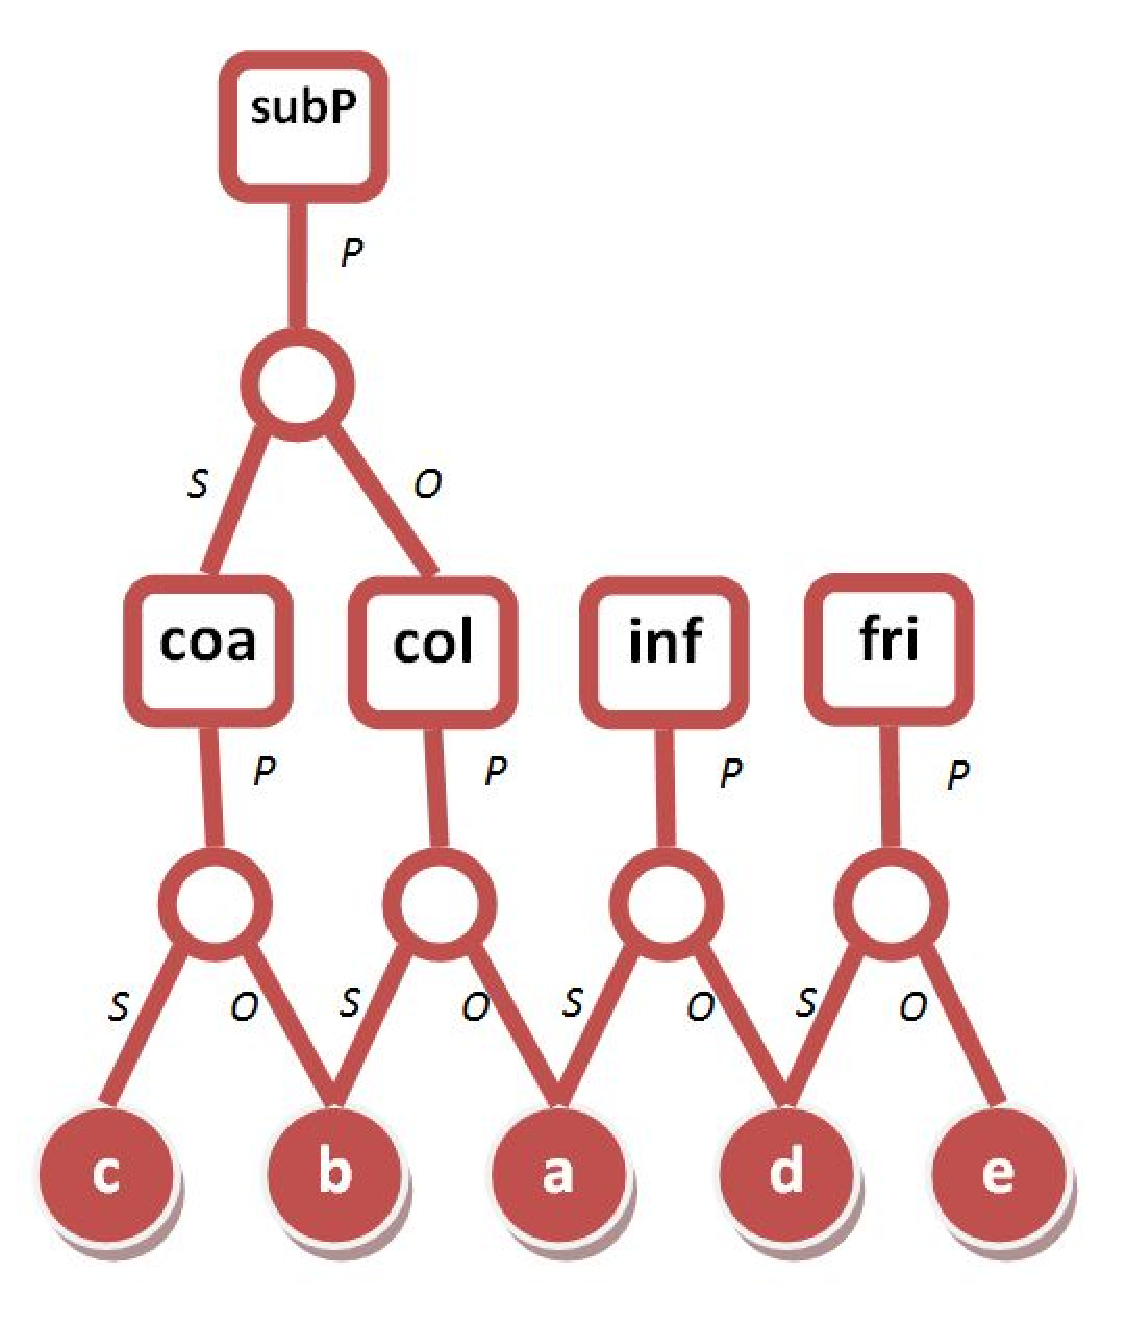
\includegraphics[width=.4\textwidth]{fig/BG.eps}
\end{center}
\caption{\label{fig:BG} .}
\end{figure}

\end{comment}

Formally, a hypergraph $G = (V,E)$, is a pair in which $V$ is the vertex set and $E$ is the hyperedge set where each $e \in E$ is a subset of $V$. A weighted hypergraph is a hypergraph that has a positive number $w(e)$ associated with each hyperedge $e$; called the weight of hyperedge $e$: Denote a weighted hypergraph by $G = (V,E,w)$. The degree of a vertex $v \in V$, $d(v)$, is defined as $d(v) = \sum_{v\in V, e\in E}{w(e)}$. The degree of a hyperedge $e$, denoted as $\delta(e)$, is the number of vertices in $e$, i.e. $\delta(e)=|e|$. A hyperedge $e$ is said to be incident with a vertex $v$ when $v \in e$. The hypergraph incidence matrix $\mathbf{H} \in \mathbb{R}^{|V| \times |E|}$ is defined as
\begin{equation}
\notag h(v,e)=\left\{\begin{array}{cl}
	   1, & v \in e \\
	   0, & otherwise
	   \end{array}\right.
\end{equation}
Throughout the rest of the dissertation, the diagonal matrix forms for $\delta(e)$, $w(e)$, $d(v)$ are denoted as $\mathbf{D}_e$, $\mathbf{W} \in \mathbb{R}^{|E|}$, and $\mathbf{D}_v \in \mathbb{Z}^{|V|}$, respectively.

\section{Graphs in Data Mining}
\subsection{Graph Representation of Relational Structure}
An object set endowed with pairwise relationships can be naturally illustrated as a graph in which vertices represent objects, and any two vertices that have some kind of relationship are joined together by an edge. In the case of frequent itemset mining, a set of objects with the co-occurrence relationship can be represented as directed or undirected graphs. For illustrating this point of view, let us consider a relational table depicted in Figure~\ref{fig:hg_and_rg}(a). One can construct an undirected graph where the set of vertices is the set of relational attributes (column items) and an edge joins two vertices if the they co-occur in a tuple (as illustrated in Figure~\ref{fig:hg_and_rg}(b)). This graph is called \emph{Gaifman graph}~\cite{Hodkinson02finiteconformal} of a relational structure. The undirected graph can be further enriched by assigning to each edge a weight equal to the support of the 2-itemset consisting of vertices incident to the edge. Cliques (complete subgraphs) in the Gaifman graph, or \emph{Gaifman cliques} for short, are of particular interest because every tuple (ground atom) in data corresponds to a Gaifman clique. However, ambiguity arises as not all Gaifman cliques have matching tuple in the data. There exists cases where cliques are incidental in the sense that several relational ground atoms play together to induce a clique configuration in the Gaifman graph, but no ground atom covers the entire clique (e.g., the clique of $\{A,B,C,D\}$ in Figure~\ref{fig:hg_and_rg}(b) does not correspond to any tuple in the relational table).

\begin{figure*}[tbh]
\begin{center}
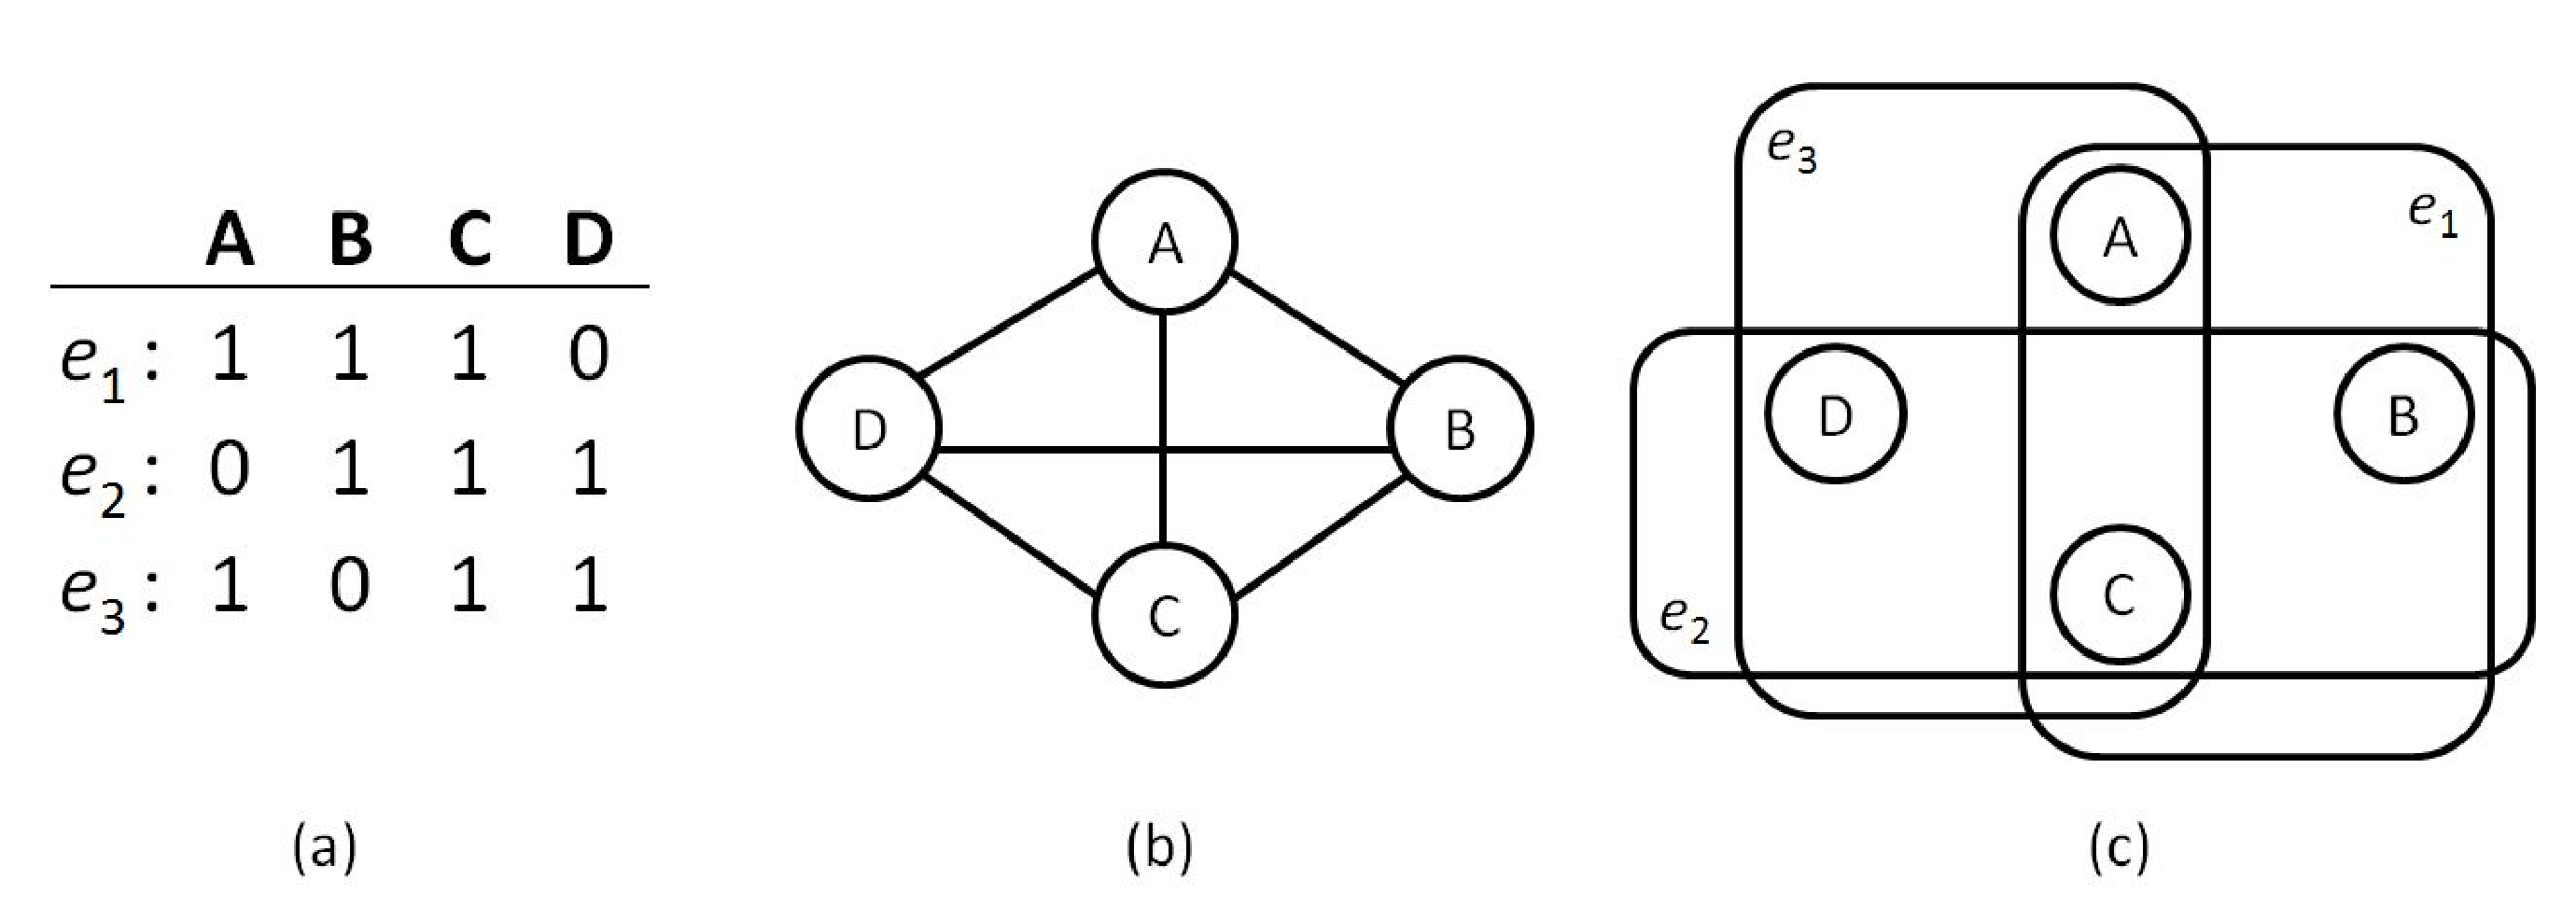
\includegraphics[width=.8\textwidth]{fig/hg_and_rg1.eps}
\end{center}
\caption[An example of simple graph vs. hypergraph for representing a relational table.]{\label{fig:hg_and_rg} (a) an example transaction table; (b) the Gaifman graph representation of the table; (c) The hypergraph representation of the table}
\end{figure*}

A natural way to remedy the ambiguity is to represent the relational data as a \emph{hypergraph}~\cite{Hypergraph}. A hypergraph is a generalization of traditional graph. An edge in the hypergraph, called hyperedge, can connect more than two vertices. In other words, every hyperedge is an arbitrary nonempty subset of vertices. It is obvious that a simple graph is a special kind of hypergraph with each hyperedge containing only two vertices. We propose to employ hypergraphs to model relational structure for finding semantically associated itemsets. Specifically, we propose to construct a hyperedge for each tuple. The relational attributes constitute the universe of vertices in the hypergraph. In this representation, each hyperedge has an exact one-to-one correspondent tuple (see Figure~\ref{fig:hg_and_rg}(c), for example).

\subsection{Similarity Measure}
%Sheth et al.~\cite{Sheth05semanticassociation} proposed a formalism for semantic association between entities in an RDF graph. Specifically, the semantic association is defined based on semantic connectivity which indicates if there exists a sequence of interconnected links between two given entities. In our study of semantically associated itemsets in transaction data, the link between entities is essentially the `co-occurrence' relationship. The semantic association according to Sheth et al's definition between transaction items $i_0$ and $i_n$ can be established by identifying a link of the form $i_0, P_c, i_1, P_c, \ldots, i_{n-1}, P_c, i_{n}$, in which $P_c$ denotes the co-occurrence property. The random walk model on hypergraph described in Section~\ref{sec:rw_hyper} formalizes this point of view. Our method for measuring the strength of semantic association is hence based on constructing a hypergraph representation and studying its property with both graph theoretical and spectral analysis techniques.

%Connectivity query between two nodes are essential in numerous mining tasks. Sheth et al.~\cite{Sheth05semanticassociation} defined semantic connectivity in RDF graph as follows. Two entities $e_1$ and $e_n$ are semantically connected if there exists a sequence $e_1, P_1, e_2, P_2, e_3, \ldots, e_{n-1}, P_{n-1}, e_n$ in an RDF graph where $e_i$ are entities and $P_j$ are properties. A sequence of alternating entities and properties represents a semantic path. Fig.~\ref{fig:graphcomp}(B) shows the connectivity between nodes c, a, and e. Paths connecting these nodes are colored in blue.

Given graph-based representation of information sources, meaningful similarity measure $s$ between nodes in the graph is critical in numerous data mining tasks. Take the simple network in Fig.~\ref{fig:graphcomp}(B) for example, suppose given a task of friend recommendation based on the information in this graph, the interesting question is whether $c$ or $e$ is a better choice of recommendation to $a$. To answer this question, it is natural to compare the similarity measures $s(a, c)$ and $s(a, e)$. In a rough sense, on can identify in the hypergraph representation that there are two paths between $a$ and $c$ (the formal definition for paths in hypergraphs will be given in Section~\ref{sec:rw_hyper}), while only one between $a$ and $e$. It's intuitive to conclude that $a$ and $c$ are more similar, or closer, than $a$ and $e$. This gives us a hint that meaningful similarity measures on the graph should satisfy the following intuitions:
\begin{enumerate}
\item The more paths connecting two nodes, the closer they are.
\item The shorter the paths, the closer they are.
\end{enumerate}
In other words, the more ``short" connections between two given nodes, the more similar those nodes are. To this end, we propose to employ the following quantities as the candidate similarity measure since both of them have the desired property. They are, namely, the \emph{commute time distance} based similarity measure from the random walk model on hypergraph, and the inner product similarity based on the \emph{pseudoinverse of the hypergraph Laplacian}. They are all based on the random walk model on hypergraph. In the following, we briefly introduce the theory of random walk.

\subsubsection{Random Walk}
\textbf{Random Walk on Simple Graph}
Given a graph and a starting point we select a neighbor of it at random and move to this neighbor then we select a neighbor of this point at random and move to it etc. The random sequence of points selected this way is a random walk on the graph. In other words, a random walker can jump from vertex to vertex and each vertex therefore represents a state of the Markov chain. The average first-passage time $m(k|i)$~\cite{randomwalks} is the average number of steps needed by a random walker for reaching state $k$ for the first time, when starting from state $i$. The symmetrized quantity $n(i,j)=m(j|i)+m(i|j)$ called the average commute time~\cite{randomwalks}, provides a distance measure between any pair of states. The fact that this quantity is indeed a distance on a graph was proved independently by Klein and Randic~\cite{Klein} and Gobel and Jagers~\cite{Gobel}.

%The average commute time has the nice property of decreasing when the number of paths connecting two vertices increases and when the ``length" of any path decreases, that is, when communication is facilitated. In short, the more short paths connect two given vertices, the more similar those vertices are. The ``shortest path" or ``geodesic" distance does not have the nice property of decreasing when connections between nodes are added: It does not capture the fact that strongly connected nodes are at a smaller distance than weakly connected ones.

The Laplacian matrix $\mathbf{L}$ of a graph is widely used for finding many properties of the graphs in spectral graph theory. Given node degree matrix $\mathbf{D}$ and graph adjacency matrix $\mathbf{A}$, the Laplacian matrix of the graph is defined as $\mathbf{L}=\mathbf{D}-\mathbf{A}$. The normalized Laplacian is given by $\mathbf{L}_N=\mathbf{I}-\mathbf{D}^{-1/2}\mathbf{A}\mathbf{D}^{-1/2}$, where $\mathbf{I}$ is the identity matrix. The average commute time $n(i,j)$ can be computed in closed form from the Moore-Penrose pseudoinverse of $\mathbf{L}$~\cite{pseudo}, denoted by $\mathbf{L}^+$.

Various quantities derived from random walk on graph has been used in a number of applications. Fouss et al.~\cite{Fouss06random-walkcomputation} compared twelve scoring algorithms based on graph representation of the database to perform collaborative movie recommendation. Pan et al.~\cite{Pan} developed a similarity measure based on random walk steady state probability to discover correlation between multimedia objects containing data of various modalities. Yen et al.~\cite{Yen05clusteringusing} introduced a new k-means clustering algorithm utilizing the random walk average commute time distance. Zhou et al.~\cite{Zhou:2009:GCB:1687627.1687709} presented a unified framework based on neighborhood random walk to integrate structural and attribute similarities for graph clustering.



\begin{comment}

The field of graph mining has seen a rapid explosion in recent years because of new applications in computational biology, software bug localization, and social and communication networking. This book is designed for studying various applications in the context of managing and mining graphs. Graph mining has been studied by the theoretical community extensively in the context of numerous problems such as graph partitioning, node clustering, matching, and connectivity analysis. However the traditional work in the theoretical community
cannot be directly used in practical applications because of the following reasons:

The definitions of problems such as graph partitioning, matching and dimensionality reduction are too ``clean" to be used with real applications. In real applications, the problem may have different variations such as a disk-resident case, a multi-graph case, or other constraints associated with the graphs. In many cases, problems such as frequent sub-graph mining and dense graph mining may have a variety of different flavors for different scenarios.

The size of the applications in real scenarios are often very large. In such cases, the graphs may not be stored in main memory, but may be available only on disk. A classic example of this is the case of web and social network graphs, which may contain millions of nodes. As a result, it is often necessary to design specialized algorithms which are sensitive to disk access efficiency constraints. In some cases, the entire graph may not be available at one time, but may be available in the form of a continuous stream. This is the case in many applications such as social and telecommunication networks in which edges are received continuously.

It is assumed that the underlying graphs are massive and cannot be held in main memory. This change in assumption has a critical
impact on the algorithms which are required to process such graphs. The problems studied in the book include algorithms for frequent pattern mining, graph matching, indexing, classification, clustering, and dense graph mining. In many cases, the problem of graph management and mining has been studied from the perspective of structured and XML data. Where possible, we have clarified the
connections with the methods and algorithms designed by the XML data management community. We also provide a detailed discussion of the application of graph mining algorithms in a number of recent applications such as graph privacy, web and social networks.

Many of the graph algorithms are sensitive to the application scenario in which they are encountered. Therefore, we will study the usage of many of these techniques in real scenarios such as the web, social networks, and biological data. This provides a better understanding of how the algorithms in the book apply to different scenarios. Thus, the book provides a comprehensive summary both from an algorithmic and applied perspective.
\end{comment}

\section{Semantic Annotation and Matching}
\label{sec:annotAndMatching}
\subsection{The Multiobjective Optimization Problem and Pareto-Optimality}
Multi-objective optimization problem (also called multi-criteria, multi-performance or vector optimization) can be defined mathematically as to find the vector $X=[x_1, x_2, \ldots, x_k]^T$ which satisfies the following $m$ inequality constraints and $l$ equality constraints:
\begin{align}
\notag g_i(X)&\geq0, i=1,2,\ldots,m\\
\notag h_i(X)&=0, i=1,2,\ldots,l
\end{align}
and optimize the objective function vector
\begin{align}
\notag F(X)=[f_1(X), f_2(X), \ldots, f_N(X)]^T
\end{align}
where $X=[x_1, x_2, \ldots, x_k]^T$ is called the decision variable vector.

%%
Real-life problems require simultaneous optimization of several incommensurable and often conflicting objectives. Usually, there is no single optimal solution, but there is a set of alternative solutions. These solutions are optimal in the sense that no other solutions in the search space are superior to each other when all the objectives are considered~\cite{SumanSurvey}. They are known as Pareto-optimal solutions. To define the concept of Pareto optimality, we take the example of a minimization problem with two decision vectors $a, b\in X$. Vector $a$ is said to dominate $b$ if
\begin{align}
\notag \forall i &= \{1,2,\ldots,N\}~:~f_i(a)\leq f_i(b)\\
\notag and\\
\notag \exists j &= \{1,2,\ldots,N\}~:~f_j(a)<f_j(b)
\end{align}
When the objectives associated with any pair of non-dominated solutions are compared, it is found that each solution is superior with respect to at least one objective. The set of non-dominated solutions to a multi-objective optimization problem is known as the Pareto-optimal set (Pareto front)~\cite{Zitzler98multiobjectiveoptimization}.

\subsubsection{Metaheuristics on Solving Multi-Objective Optimization Problems}
Metaheuristics are used for combinatorial optimization in which an optimal solution is sought over a large, discrete search-space. Popular metaheuristics for combinatorial problems include simulated annealing by Kirkpatrick et al.~\cite{Kirkpatrick1987}, genetic algorithms by Holland et al.\cite{Holland1992}. Extensive previous research has been devoted to extend these methods to multi-objective optimization problems as discussed in the following, which yield sets of mutually non-dominating solutions that are an approximation to the true Pareto front. In Section~\ref{sec:method} we explore in detail the multi-objective simulated annealing algorithm applied to the dual matching problem. We compare the performance with the multi-object genetic algorithm in Section~\ref{sec:experiment}.

\textbf{Simulated Annealing in Multi-Objective Optimization:} Simulated annealing (SA) is based on an analogy of thermodynamics with the way metals cool and anneal. It has been proved to be a compact and robust technique. Simulated Annealing was started as a method or tool for solving single objective combinatorial problems, these days it has been applied to solve single as well as multiple objective optimization problems in various fields. A comprehensive survey can be found in~\cite{SumanSurvey}.

\textbf{Evolutionary Multi-Objective Optimization:} Evolutionary multi-objective optimization covers the use of many types of heuristic optimizers inspired by the natural process of evolution. As in nature, a population of individuals (solutions to the problem) exist and, through a process of change and competition between these individuals, the quality of the population is advanced. Deb~\cite{Deb2001} provides an introduction of evolutionary algorithms (e.g., genetic algorithm) for multi-objective as the state of the art.

\subsection{The Schema Matching Problem}
Our study of matching alternative attribute sets is closely related to the schema matching problem in data integration. According to the type of instance value, various instance-based approaches have been developed in previous research. For example, for textual attributes, a linguistic characterization based on information retrieval techniques can be applied~\cite{Rahm01asurvey}; for nominal attributes, evaluation of the degree of overlap of instance values is a preferred approach. Larson et al.~\cite{Larson1989} and Sheth et al.~\cite{Sheth1988} discussed how relationships and entity sets could be integrated primarily based on their domain relationships. Similarity of partially overlapped instance set can be also calculated based on measures such as Hamming distance and Jaccard coefficient; for numeric attributes, most methods use aggregated statistics to characterize the attributes, e.g., `SSN' and `PhonNo' can be distinguished based on their respective patterns~\cite{Rahm01asurvey}. Hybrid systems that combine several approaches to determine matching often achieve better performance. For example, SemInt~\cite{Li00semint:a} is a comprehensive matching prototype exploiting up to 15 constraint-based and 5 content-based matching criteria. The LSD (Learning Source Descriptions)~\cite{Doan2000} system uses several instance-level matchers (learners) that are trained during a preprocessing step. The iMAP~\cite{Dhamankar04imap} system uses multiple basic matchers, called searches, e.g., text, numeric, category, unit conversion, each of which addresses a particular subset of the match space.

Due to the nature of many scientific datasets, we face several unique challenges. First, the data under study is semi-structured, thus invalidating those matching methods that presume a complete, known-in-advance schematic structure. In addition, totally different labels (usually acronyms or pseudowords) are widely adopted for the same or similar metrics, rendering lexical similarity-based methods unsuitable. Moreover, an important limitation of previous instance-based matching methods is their inability to handle numerical instances appropriately in certain domain applications. They use statistical characterization extracted from the numerical instances, such as range, mean and standard deviation, to determine match. However such information is too rough to capture patterns in data that are crucial in determining the correspondence.

\subsection{The Cluster Matching Problem}
\label{sec:clusterMatching}
\emph{Density Profile}: To represent clusters using density profiles, the attribute's range in each cluster is first discretized into a number of bins, and the similarity between two clusters corresponds to the number of points of each cluster falling within these bins. The formal definition for this number of points is the \textit{density} of an attribute-bin region for cluster $c_k$ in clustering $C$, denoted as $dens_C(k, i, j)$. It refers to the number of points in the region $(i, j)$---the $j$-th bin of the $i$-th attribute---that belongs to the cluster $c_k$ of clustering $C$. For example, for clustering $C$ in Fig.~\ref{fig:density_profile}, $dens_C(1, 1, 1) = 8$, because there are 8 data points in region $(1, 1)$---the first bin of the first attribute $x$---that belongs to the first cluster $c_1$.

%The values of $dens_C(k, i, j)$ for all possible $k$, $i$, $j$ are then listed in a certain ordering to form a clustering's \emph{density profile vector} (defined below). This ordering is imposed on all attribute-bin regions and must be applied to the two datasets in which the clusterings were generated. It is necessary, then, that both datasets must have the same attribute set. If this requirement does not stand, the matching between the sets must be specified in advance. Therefore, in order to apply the density profile method in the ERP pattern matching problem, we must first carry out measure matching. We further discuss the interdependence between pattern matching and metric matching in Section~\ref{sec:discuss}.

The density profile vector $V_C$ for a clustering $C$ is formally defined as an ordered tuple:
\begin{align}
\notag V_C = \bigg[ & dens_C(1, 1, 1), ~\ldots, ~dens_C (1, 1, Q),\\
\notag & dens_C (1, 2, 1), ~\ldots, ~dens_C (1, M, Q),\\
& dens_C (2, 1, 1), ~\ldots, ~dens_C (N, M, Q) \bigg]\, ,\label{eq:densp}
\end{align}
where $Q$ is the number of bins in each of the $M$ attributes, and $N$ is the number of clusters in $C$.

\emph{The ADCO measure}: After the density profile vectors of two clusterings $C$ and $C'$ are obtained, the degree of similarity between  $C$ and $C'$ can be determined by calculating the dot product of the density profile vectors:
$sim(C, C') = V_C  \cdot V_{C'} \, .$

The $ADCO(C,C')$ measure is defined as $sim(C,C')$ normalized by the maximum achievable similarity when using either of the two clusterings:
\begin{equation}
ADCO(C, C') = \frac{sim(C, C')}{NF(C, C')} \, , \label{eq:adco}
\end{equation}
where $NF(C, C') = max \big[sim(C, C), \,sim(C', C')\big]$.

\begin{figure}[tb]
\begin{center}
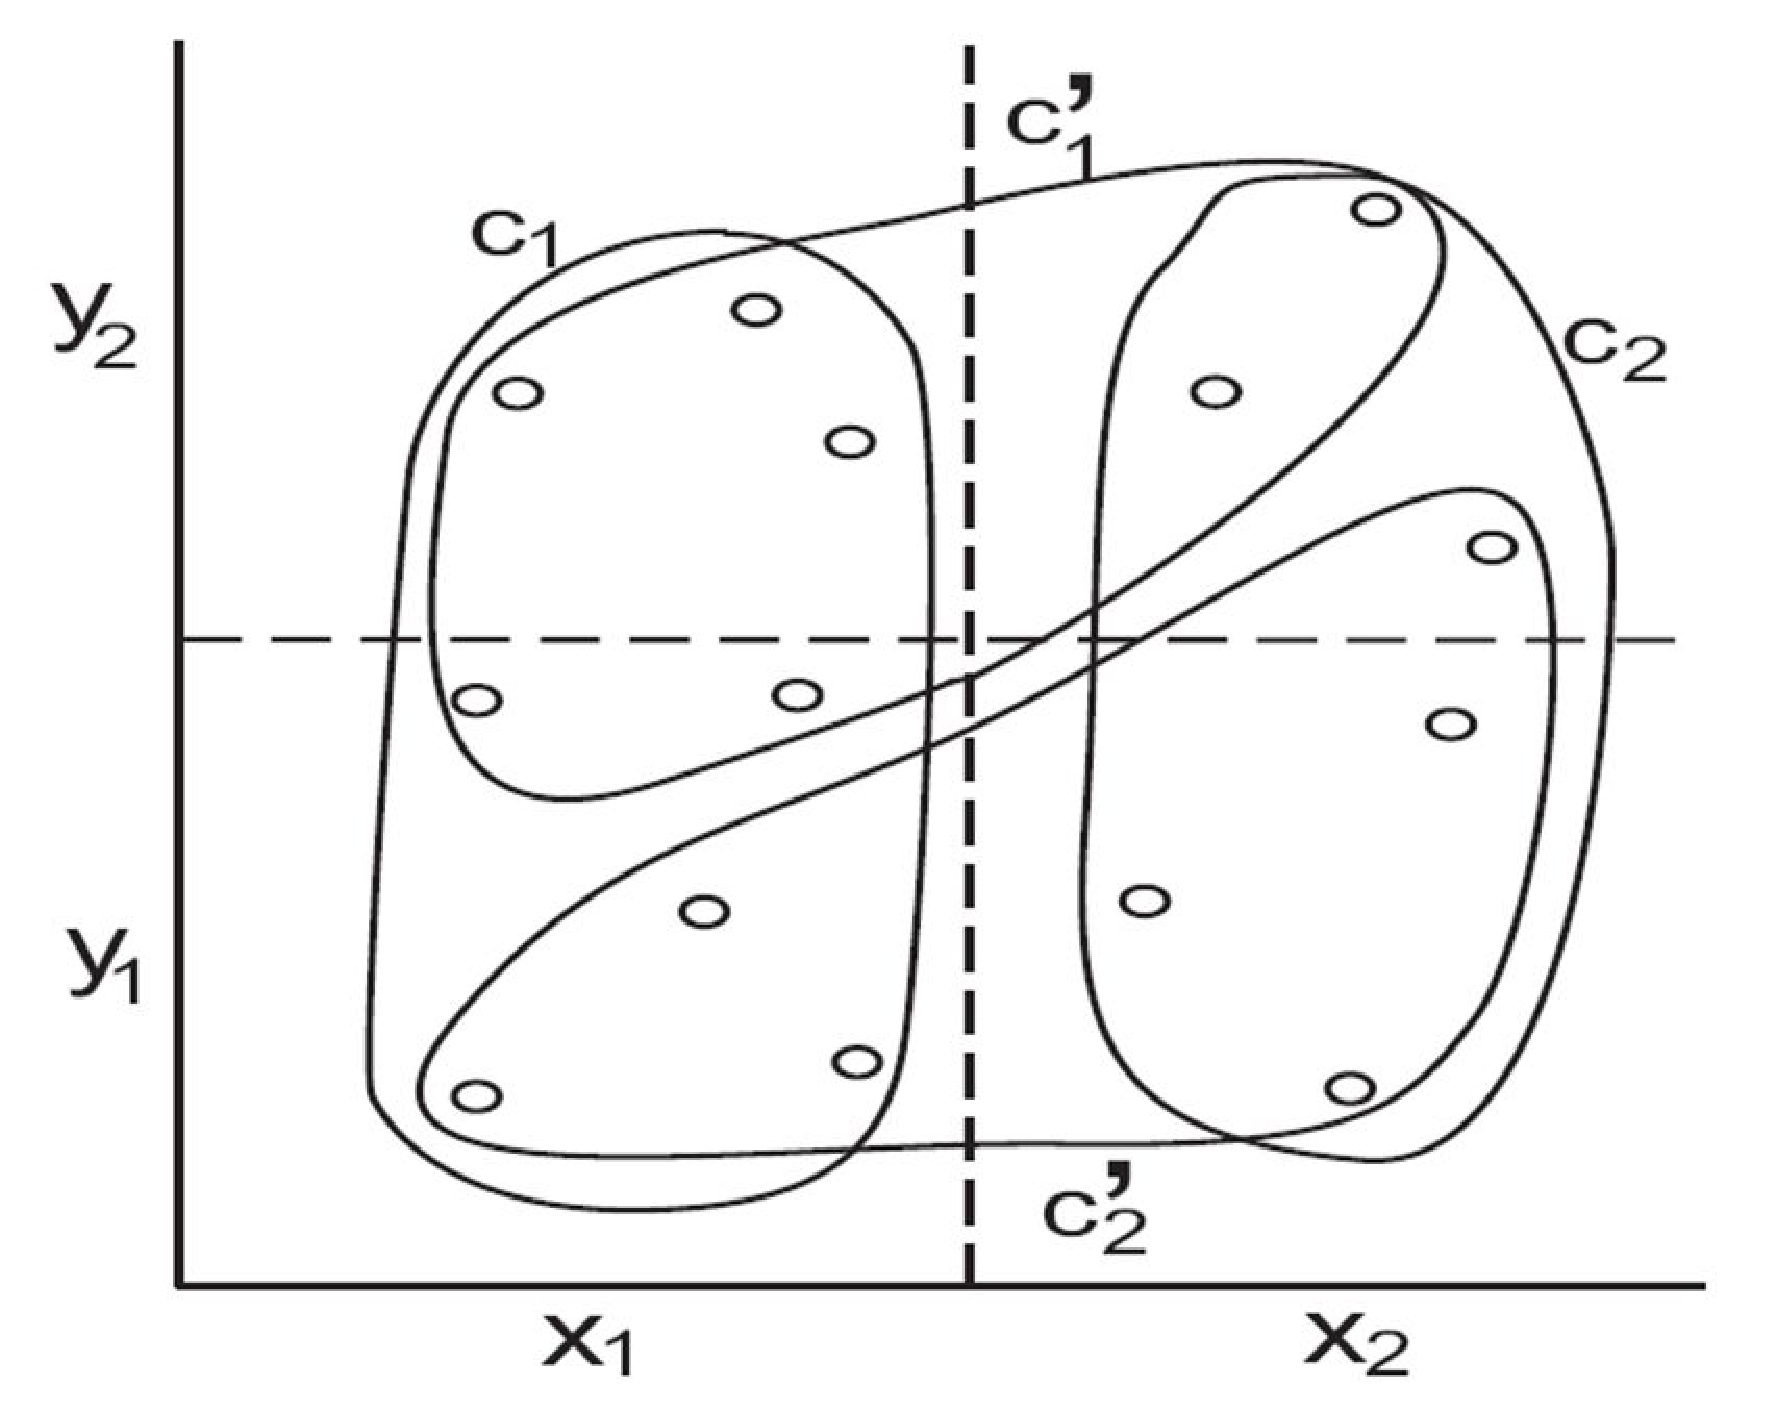
\includegraphics[width=0.4\textwidth]{fig/density_profile.eps}
\end{center}
\caption[An example of cluster density profiles]{\label{fig:density_profile} Two clusterings $C=\{c_1, c_2\}$ and $C'=\{c_1', c_2'\}$. Two attributes $X$ (attribute 1) and $Y$ (attribute 2) are discretized into 2 bins each. See~\cite{Bae2010} for details.}
\end{figure} 

\subsection{Collective Classification for Schema and Data Matching}
Collective classification in relational data has become an important and active research topic in the last decade, where class labels for a group of linked instances are correlated and need to be predicted simultaneously~\cite{kong:multi-label}. It has been applied to tackle multiple integration problems that are traditionally solved independently. Wick et al.~\cite{Wick2008} describe a discriminatively-trained model based on Markov random field to perform joint reasoning about schema matching, coreference, and canonicalization. Namata et al.~\cite{Namata2011} proposed an approach consisting of coupled collective classifiers to discover a latent graph structure underlying an observed one by addressing entity resolution, link prediction, and node labeling simultaneously. The difference between these previous methods and our proposed method mainly lies in the fact that we do not require a training phase. Instead, the matchings are discovered by simultaneously optimizing interrelated objective functions which circumvents the labor for acquiring labeled data and the expense of statistical inference.

Last but not least, we have made important extensions in this paper compared with our conference paper version~\cite{LiuDou11}. In this paper, we implement an evolutionary multi-objective approach as the metaheuristics algorithm to discover attribute and cluster matching. We have also conducted more experiments on real-world datasets to demonstrate the utility of the proposed method.

